\chapter{Metodologie e Modelli per il progetto}



\section{Introduzione alla progettazione}

\subsection{Il ciclo di vita dei sistemi informativi}
La progettazine di una base di dati costituisce solo una delle componenti del processo di sviluppo di un sistema informativo, e va quindi inserita in un contesto più ampio, quello del \textbf{ciclo di vita} di un sistema informatico.\\\\
Il ciclo di vita di un sistema informativo comprende, generalmente, le seguenti attività:
    \begin{itemize}
        \item{\textbf{Studio di fattibilità}: serve a definire, in maniera per quanto possibile precisa, i costi delle varie alternative possibili e a stabilire le priorità di realizzazione delle varie componenti del sistema.}
        \item{\textbf{Raccolta e analisi dei requisiti}: consiste nell'individuazione e nello studio delle proprietà e delle funzionalità che il sistema informativo dovrà avere.\\
        Questa fase richiede un'interazione con gli utenti del sistema e produce una descrizione completa, ma generalmente informale, dei dati coinvolti (anche in termini di previsione sul carico applicativo) e delle operazioni su di essi (anche in termini di previsione della loro frequenza).\\
        Vengono inoltre stabiliti i requisiti software e hardware del sistema informativo.}
        \item{\textbf{Progettazione}: si divide generalmente in \textbf{progettazione dei dati} e \textbf{progettazione delle applicazioni}.\\
        Nella prima si individua la struttura e l'organizzazione che i dati dovranno avere, nell'altra si definiscono le caratteristiche dei programmi applicativi.\\
        Le due attività sono complementari e possono procedere in parallelo o in cascata.\\
        Le descrizioni dei dati e delle applicazioni prodotte in questa fase sono formali e fanno riferimento a specifici modelli.}
        \item{\textbf{Implementazione}: consiste nella realizzazione del sistema informativo secondo la struttura e le caratteristiche definite nella fase di progettazione.\\
        Viene costruita e popolata la base di dati e viene prodotto il codice dei programmi.}
        \item{\textbf{Validazione e collaudo}: serve a verificare il corretto funzionamento e la qualità del sistema informativo.\\
        La sperimentazione deve prevedere, per quanto possibile, tutte le condizioni operative.}
        \item{\textbf{Funzionamento}: in questa fase il sistema informativo diventa operativo ed esegue i compiti per i quali era stato originariamente progettato.\\
        Se non si verificano malfunzionamenti o revisioni delle funzionalità del sistema, questa attività richiede solo operazioni di gestione e manutenzione.}
    \end{itemize}
Il processo non è quasi mai strettamente sequenziale in quanto, spesso, durante l'esecuzione di una delle attività citate, bisogna rivedere decisioni prese nell'attività precedente. Si ottiene proprio un \textbf{ciclo} di operazioni.\\
Inoltre, si aggiunge talvolta alle attività citate quella di \textbf{prototipazzione}, che consiste nell'uso di specifici strumenti software per la realizzazione rapida di una versione semplificata del sistema informativo.\\\\
Le basi di dati costituiscono in effetti solo una delle componenti del sistema, ma il loro ruolo centrale i dati hanno in un sistema informativo giustifica uno studio autonomo relativo alla \textbf{progettazione delle basi di dati}.\\
Ci interesseremo solo agli aspetti dello sviluppo dei sistemi informativi che riguardano da vicino il progetto delle basi di dati, focalizzando l'attenzione in particolare sulla terza fase del ciclo, discutendo anche alcuni aspetti riguardanti l'attività di raccolta e analisi dei dati.\\\\
Questa maniera di procedere è coerente con l'approccio allo sviluppo dei sistemi informativi basato sui dati, in cui l'attenzione è centrata sui dati e sulle loro proprietà.\\
Questo approccio prevede prima la progettazione della base di dati e, successivamente, la realizzazione delle applicazioni che la utilizzano.

\subsection{Metodologie di progettazione e basi di dati}
Un aspetto che vale la pena di precisare è che cosa si intende per \textbf{metodologia di progettazione} e quali sono le priorità che una metodologia deve garantire.\\
In buona sostanza, una metodologia di progettazione consiste in:
    \begin{itemize}
        \item{Una \textbf{decomposizione} dell'intera attività di progetto in passi successivi indipendenti tra loro.}
        \item{Una serie di \textbf{strategie} da seguire nei vari passi e alcuni \textbf{criteri} per la scelta in caso di alternative.}
        \item{Alcuni \textbf{modelli di riferimento} per descrivere i dati di ingresso e uscita delle varie fasi.}
    \end{itemize}
Le proprietà che una metodologia deve garantire sono principalmente:
    \begin{itemize}
        \item{La \textbf{generalità} rispetto alle applicazioni e ai sistemi in gioco (e quindi la possibilità di utilizzo indipendentemente dal problema allo studio e dagli strumenti a disposizione).}
        \item{La \textbf{qualità del prodotto} in termini di correttezza, competezza ed efficienza rispetto alle risorse impiegate.}
        \item{La \textbf{facilità d'uso} delle strategie e dei modelli di riferimento.}
    \end{itemize}
Nell'ambito delle basi di dati si è consolidata negli anni una metodologia di progetto che ha dato prova di soddisfare pienamente queste tre proprietà.\\
Tale metodologia è articolata in tre fasi principali da effettuare in cascata e si fonda sul seguente principio: separare in maniera netta le decisioni relative a \textit{cosa} rappresentare in una base di dati (prima fase), da quelle relative a \textit{come} farlo (seconda e terza fase).
    \begin{itemize}
        \item{\textbf{Progettazione concettuale}: in questa fase rappresentiamo le specifiche informali della realtà di interesse in termini di una descrizione formale e completa, ma indipendente dai criteri di rappresentazione utilizzati nei sistemi di gestione di basi di dati.\\
        Il prodotto di questa fase è detto \textbf{schema concettuale} e fa riferimento a un \textbf{modello concettuale} dei dati.\\
        I modelli concettuali ci permettono di descrivere l'organizzazione dei dati a un alto livello di astrazione, senza tenere conto degli aspetti implementativi.\\
        In questa fase, infatti, il progettista deve cercare di rappresentare il \textbf{contenuto informativo} della base di dati, senza occuparsi né delle modalità con le quali queste informazioni verranno codificare in un sistema reale, né dell'efficienza dei programmi che faranno uso di queste informazioni.}
        \item{\textbf{Progettazione logica}: in questa fase traduciamo lo schema concettuale definito nella fase precedente, in termini del modello di rappresentazione dei dati adottato dal sistema di gestione di base di dati a disposizione.\\
        Il prodotto di questa fase viene denominato \textbf{schema logico} della base di dati e fa riferimento a un \textbf{modello logico} dei dati.\\
        Un modello logico ci permette di descrivere i dati secondo una rappresentazione ancora indipendente dai dettagli fisici, ma concreta perché disponibile nei sistemi di gestione di base di dati.\\
        In questa fase, le scelte progettuali si basano, tra l'altro, su criteri di ottimizzazione delle operazioni da effettuare sui dati.\\
        Si fa comunemente uso anche di tecniche formali di verifica della qualità dello schema logico ottenuto. Nel caso del modello relazionale dei dati, la tecnica comunemente utilizzata è quella della \textbf{normalizzazione}.}
        \item{\textbf{Progettazione fisica}: in questa fase lo schema logico viene completato con la specifica dei parametri fisici di memorizzazione dei dati (organizzazione dei file e degli indici).\\
        Il prodotto di questa fase viene denominato \textbf{schema fisico} e fa riferimento a un \textbf{modello fisico} dei dati.}
    \end{itemize}
È necessario fare una distinzione tra \textbf{specifiche sui dati}, che riguardano il contenuto della base di dati, e \textbf{specifiche sulle operazioni}, che riguardano l'uso che utenti e applicazioni fanno della base di dati.\\\\
Nella progettazione concettuale si fa uso soprattutto delle specifiche sui dati, mentre le specifiche sulle operazioni servono solo a verificare che lo schema concettuale sia completo, contenga cioè le informazioni necessarie per eseguire tutte le operazioni previste.\\\\
Nella progettazione logica, invece, lo schema concettuale in ingresso riassume le specifiche sui dati, mentre le specifiche sulle operazioni si utilizzano, insieme alle previsioni sul carico applicativo, per ottenere uno schema logico che renda tali operazioni eseguibili in maniera efficiente.\\
In questa fase bisogna anche conoscere il modello logico adottato, ma non è ancora necessario conoscere il particolare DBMS scelto (solo la categoria cui appartiene).\\
Infine, nella progettazione fisica si fa uso dello schema logico e delle specifiche sulle operazioni per ottimizzare le prestazioni del sistema.\\
In questa fase è necessario anche tenere conto delle caratteristiche del particolare sistema di gestione di basi di dati utilizzato.\\\\
Il risultato della progettazione di una base di dati non è solo lo schema fisico, ma è costituito anche dallo schema concettuale e dallo schema logico.\\
Lo schema concettuale fornisce infatti una rappresentazione della base di dati di alto livello, che può essere molto utile a scopo documentativo, mentre lo schema logico fornisce una descrizione concreta del contenuto della base di dati che, prescindendo dagli aspetti implementativi, è il riferimento per le operazioni di interrogazione e aggiornamento.\\\\
Nel caso della progettazione di una base di dati relazionale basata sull'uso del più diffuso modello concettuale dei dati, il modello Entità-Relazione.\\
A partire da requisiti rappresentati da documenti e moduli di vario genere, acquisiti anche attraverso l'interazione con gli utenti, viene costruito uno schema E-R che descrive a livello concettuale la base di dati.\\
Questa rappresentazione viene poi tradotta in uno schema relazionale, costituito da una collezione di tabelle.\\
Infine, i dati vengono descritti da un punto di vista fisico (tipo e dimensione dei vari campi) e vengono specificate strutture ausiliarie, come gli indici, per l'accesso efficiente ai dati.



\section{Il modello E-R}
Il modello Entità-Relazione è un \textbf{modello concettuale} di dati, e, come tale, fornisce una serie di strutture, dette \textbf{costrutti}, atte a descrivere la realtà d'interesse in una maniera facile da comprendere e che prescinde dai criteri di organizzazione dei dati nei calcolatori.\\
Questi costrutti vengono utilizzati per definire \textbf{schemi} che descrivono l'organizzazione e la struttura delle \textbf{occorrenze} dei dati, ovvero, dei valori assunti al variare del tempo.\\\\
I costrutti del modello E-R sono presentati nella tabella 14.1.
    \begin{table}\caption{Costrutti del modello ER}
        \begin{center}\begin{tabular}{|c|c|} \hline
        \textbf{Costrutti} & \textbf{Rappresentazione grafica}\\ \hline
        Entità & 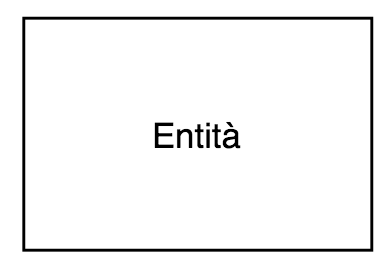
\includegraphics[scale = 0.4]{13/img0}  \\ \hline
        Relazione & 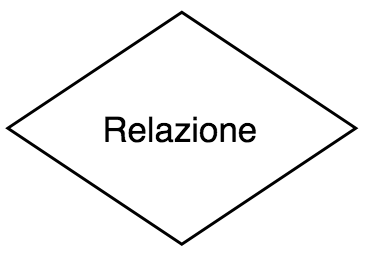
\includegraphics[scale = 0.4]{13/img1}  \\ \hline
        Attributo semplice & 
\includegraphics[scale = 0.4]{13/img2}  \\ \hline
        Attributo composto & 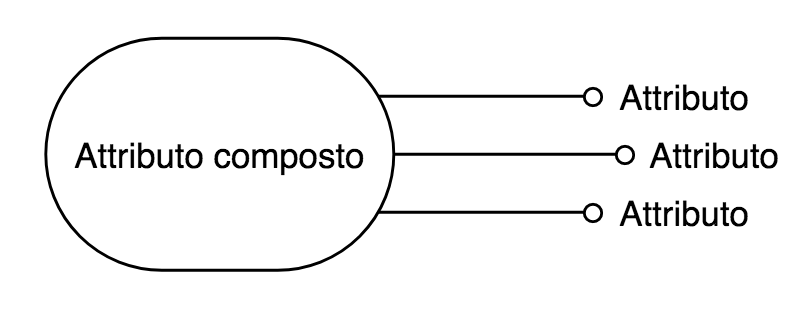
\includegraphics[scale = 0.4]{13/img3}  \\ \hline
        Cardinalità di relazione & 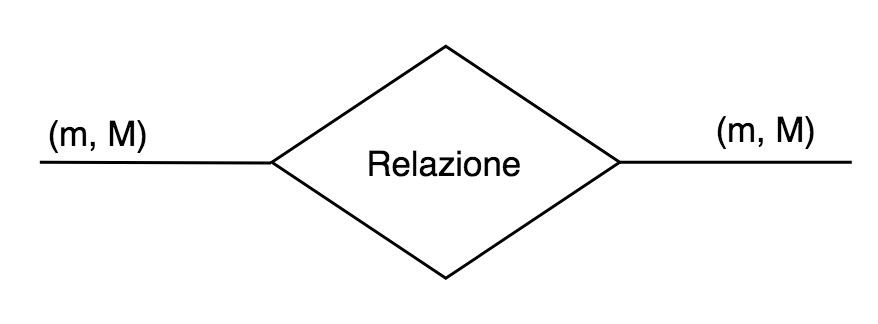
\includegraphics[scale = 0.4]{13/img4}  \\ \hline
        Cardinalità di attributo & 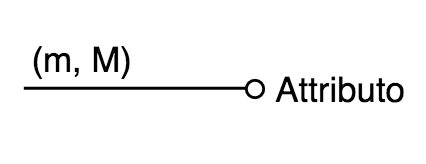
\includegraphics[scale = 0.4]{13/img5}  \\ \hline
        Identificatore interno & 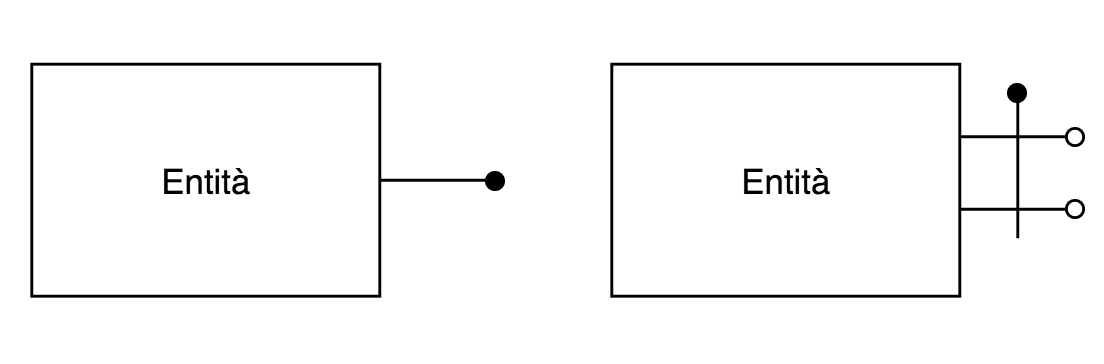
\includegraphics[scale = 0.4]{13/img6}  \\ \hline
        Identificatore esterno & 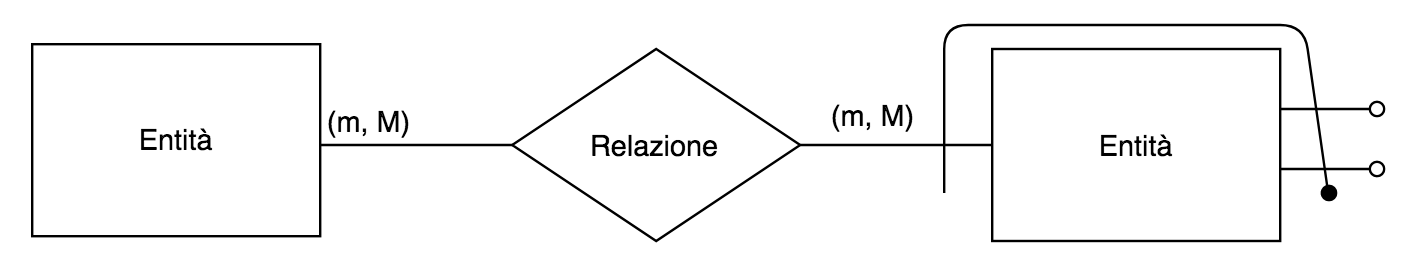
\includegraphics[scale = 0.4]{13/img7}  \\ \hline
        Generalizzazione & 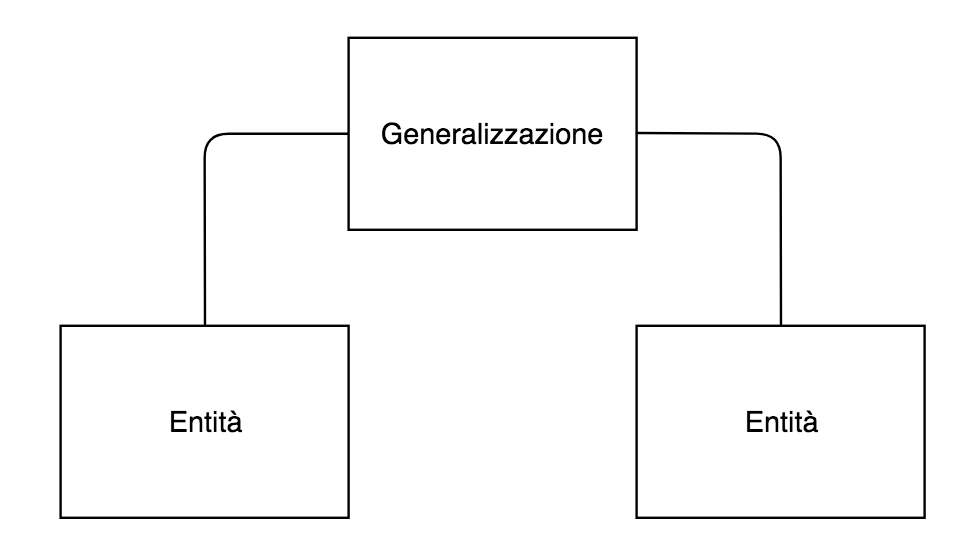
\includegraphics[scale = 0.4]{13/img8}  \\ \hline
        \end{tabular}\end{center}
    \end{table}

\subsection{I costrutti principali del modello}
\textbf{Entità.} Rappresentano classi di oggetti (es. fatti, cose, persone) che hanno proprietà comuni ed esistenza "autonoma" ai fini dell'applicazione d'interesse.\\
Si osservi che un'occorrenza di entità non è un valore che identifica un oggetto, ma è l'oggetto stesso.\\
Un'interessante conseguenza di questo fatto è che un'occorrenza di entità ha un'esistenza (e un'identità) indipendente dalle proprietà ad esso associate.\\
In questo il modello E-R presenta una marcata differenza rispetto al modello relazionale nel quale non possiamo rappresentare un oggetto senza conoscre alcune sue proprietà.\\
In uno schema, ogni entità ha un nome che la identifica univocamente e viene rappresentata graficamente mediante un rettangono con il nome dell'entità all'interno.\\\\
\textbf{Relazioni.} Rappresentano legami logici, significativi per l'applicazione d'interesse tra due o più entità.\\
Un'occorrenza di relazione è un'ennupla (coppia nel caso di relazione binaria) costituita da occorrenze di entità, una per ciascuna delle entità coinvolte.\\
In uno schema E-R, ogni relazione ha un nome che la identifica univocamente e viene rappresentata graficamente mediante un rombo, con il nome della relazione all'interno, e da linee che connettono la relazione con ciascuna delle sue componenti.\\
Possono esistere diverse che coinvolgono le stesse entità (E.G. \texttt{IMPIEGATO} e \texttt{CITTA'} possono essere in relazione \texttt{SEDE} oppure \texttt{RESIDENZA}).\\
Nella scelta dei nomi di relazione è preferibile utilizzare sostantivi invece che verbi, in maniera da non indurre ad assegnare un "verso" alla relazione. (E.g. \texttt{SEDE DI LAVORO} è preferibile a \texttt{LAVORA IN}).\\
L'insieme delle occorrenze di una relazione del modello E-R è, a tutti gli effetti, una relazione matematica tra le occorrenze delle entità coinvolte, ossia, è un sottoinsieme del loro prodotto cartesiano.\\
Questo significa che tra le occorrenze di una relazione del modello E-R non ci possono essere ennuple ripetute.\\
È anche possibile avere relazioni \textbf{ricorsive}, ovver relazioni tra un'entità e se stessa.\\
È infine possibile avere relazioni $n$-arie, relazioni, cioè, che coinvolgono più di due entità.\\\\
\textbf{Attributi.} Descrivono le proprietà elementari di entità o relazioni che sono di interesse ai fini dell'applicazione.\\
Un attributo associa a ciascuna occorrenza di entità (o di relazione) un valore appartenente a un insieme, detto \textbf{dominio}. che contiene i valori ammissibili per l'attributo. I domini non vengono riportati nello schema, ma sono generalmente descritti nella documentazione associata.\\
Può risultare comodo, qualche volta, raggruppare attributi di una medesima entità o relazione che presentano affinità nel loro significato o uso: l'insieme di attributi che si ottiene in questa maniera viene detto \textbf{attributo composto}. Per ridurre la complessità degli schemi, gli attributi commposti verranno usati raramente nel seguito preferendo usare, per quanto possibile, attributi atomici.\\\\
\textbf{Cardinalità delle relazioni.} Vengono specificate per ciascuna partecipazione di entità a una relazione e descrivono il numero minimo e massimo di occorrenze di relazione a cui una occorrenza dell'entità può partecipare. Dicono quindi quante volte, in una relazione tra entità, un'occorrenza di una di queste entità può essere legata a occorrenze delle altre entità coinvolte.\\
\textbf{E.G.:} se in una relazione \texttt{ASSEGNAMENTO} tra due entità \texttt{IMPIEGATO} e \texttt{INCARICO} specifichiamo per la prima entità una cardinalità minima 1 a 1 e una cardinalità massima pari a 5, vogliamo indicare che un impiegato può partecipare a un minimo di 1 occorrenza e a un massimo di 5 occorrenze della relazione \texttt{ASSEGNAMENTO}.\\
In linea di principio è possibile assegnare un qualunque intero non negativo a una cardinalità di una relazione con l'unico vincolo che la cardinalità minima deve essere minore o uguale della cardinalità massima. In realtà, nella maggior parte dei casi, è sufficiente utilizzare solo tre valori: zero, uno e il simbolo $N$ (che indica genericamente un intero maggiore di uno). In particolare:
    \begin{itemize}
        \item{Per la cardinalità minima, zero o uno: nel primo caso si dice che la partecipazione dell'entità relativa è \textbf{opzionale}, nel secondo si dice che la partecipazione è \textbf{obbligatoria}.}
        \item{Per la cardinalità massima, uno o molti ($N$): nel primo caso la partecipazione dell'entità relativa può essere vista come una funzione (parziale se la cardinalità minima vale zero) che associa a un'occorrenza dell'entità una sola occorrenza (o nessuna) dell'altra entità che partecipa alla relazione; nel secondo, invece, c'è un'associazione con un numero arbitrario di occorrenze dell'altra entità.}    
    \end{itemize}
Osservando le cardinalità massime, è possibile classificare le relazioni binarie in base al tipo di corrispondenza che viene stabilita tra le occorrenze delle entità coinvolte:  
    \begin{itemize}
        \item{Le relazioni aventi cardinalità massima pari a uno per entrambe le entità coinvolte definiscono una corrispondenza uno a uno tra le occorrenze di tali entità e vengono quindi denominate \textbf{relazioni uno a uno}.}
        \item{Le relazioni aventi un'entità cardinalità massima pari a uno e l'altra con cardinalità massima pari a $N$ sono denominate \textbf{relazioni uno a molti}.}
        \item{Le relazioni aventi cardinalità massima pari a $N$ per entrambe le entità coinvolte, vengono denominate \textbf{relazioni molti a molti}.}
    \end{itemize}
Per le cardinalità minime, invece, è importante notare che il caso di partecipazione obbligatoria per tutte le entità coinvolte è piuttosto raro, perché quando si aggiunge una nuova occorrenza di entità molto spesso non sono note (o addirittura non esistono) le corrispondenti occorrenze delle entità a esse collegate.\\
Le relazioni non sono necessariamente binarie, possono coinvolgere $n$ attributi, e in tal caso sono dette $n$-arie. Nelle relazioni $n$-arie le entità coinvolte partecipano quasi sempre con cardinalità massima pari a $N$.\\
Nel caso in cui un'entità partecipa a una relazione $n$-aria con cardinalità massima pari a uno, significa che ogni sua occorrenza può essere legata a una sola occorrenza della relazione e quindi a un'unica ennupla di occorrenze delle altre entità coinvolte nella relazione. Questo significa che è possibile (e risulta a volte più naturale) eliminare la relazione $n$-aria e legare direttamente tale entità con altre entità, mediante delle relazioni binarie di tipo uno a molti.\\\\
\textbf{Cardinalità degli attributi.} Possono essere specificate per gli attributi di entità o relazioni e descrivono il numero minimo e massimo di valori dell'attributo associati a ogni occorrenza di entità o relazione. Nella maggior parte dei casi, la cardinalità di un attributo è pari a $(1,1)$ e viene omessa. In questi casi l'attributo rappresenta sostanzialmente una funzione che associa a ogni occorrenza di entità un solo valore dell'attributo.\\
Il valore per un certo attributo può essere però nullo, oppure possono esistere diversi valori di un certo attributo per un'occorrenza di entità. Queste situazioni si possono rappresentare associando all'attributo in questione una cardinalità minima pari a zero nel primo caso e una cardinalità massima pari a $N$, nel secondo.\\
In maniera simile alle partecipazioni delle occorrenze di entità alle relazioni, diremo che un attributo con cardinalità minima pari a zero è \textbf{opzionale} per la relativa entità o relazione, mentre è \textbf{obbligatorio} se la cardinalità minima è pari a uno. Diremo che un attributo è \textbf{multivalore} se la sua cardinalità massima è pari a $N$.\\
In molte situazioni reali accade che certe informazioni non sono disponibili, ed è quindi utile avere la possibilità di specificare attributi opzionali. Gli attributi multivalore vanno invece utilizzati con maggiore cautela, perché essi rappresentano situazioni che possono essere modellate, in alcune occasioni con entità a sé, legate da relazioni uno a molti (o molti a molti) con l'entità cui si riferiscono.\\\\ 
\textbf{Identificatori delle entità.} Vengono specificati per ciascuna entità di uno schema e descrivono i concetti (attributi e/o entità) dello schema che permettono di identificare in maniera univoca le occorrenze delle entità. 
    \begin{itemize}
        \item{In molti casi uno o più attributi di un'entità sono sufficienti a individuare un identificatore: si parla in questo caso di \textbf{identificatore interno} (detto anche \textbf{chiave}).\\
        \textbf{E.G.:} un identificatore interno per l'entità \texttt{AUTOMOBILE} con attributi \texttt{Targa, Colore, Modello} è l'attributo \texttt{Targa}, in quanto non possono esistere due automobili con la stessa \texttt{Targa}.}
        \item{Alcune volte, però, gli attributi di un'entità non sono sufficienti a identificare univocamente le sue occorrenze.\\
        \textbf{E.G.:} Consideriamo l'entità \texttt{STUDENTE}: potrebbe sembrare, a prima vista, che l'attributo \texttt{Matricola} possa essere un identificatore per tale entità, ma ciò non è vero: studenti iscritti a università diverse possono avere lo stesso numero di matricola. Per identificare univocamente uno studente serve, oltre al numero di matricola, anche la relativa università. Quindi, un identificatore corretto per l'entità \texttt{STUDENTE} è costituito dall'attributo \texttt{Matricola} e dell'entità \texttt{UNIVERSITA'}.\\
        Osserviamo che un'entità $E$ può essere identificata da altre entità solo se tali entità sono coinvolte in una relazione a cui $E$ partecipa con cardinalità $(1, 1)$. Nei casi in cui l'identificazione di un'entità è ottenuta utilizzando altre entità si parla di \textbf{identificatore esterno}.\\
        \textbf{E.G.:} Nell'esempio precedente, l'identificazione è resa possibile dalla relazione uno a molti tra le entità \texttt{UNIVERSITA'} e \texttt{STUDENTE}, che associa a ogni studente una e una sola università. Se questa relazione non esistesse, l'identificazione univoca attraverso un'altra entità non sarebbe possibile.}
    \end{itemize}
Sulla base di quanto detto sugli identificatori, è possibile fare alcune considerazioni generali:
    \begin{itemize}
        \item{Un identificatore può coinvolgere uno o più attributi, ognuno dei quali deve avere cardinalità $(1,1)$}
        \item{Un'identificazione esterna può coinvolgere una o più entità, ognuna delle quali deve essere membro di una relazione alla quale l'entità da identificare partecipa con cardinalità $(1,1)$}
        \item{Un'identificazione esterna può coinvolgere un'entità che è a sua volta identificata esternamente, purché non vengano generati, in questa maniera, cicli di identificazioni esterne.}
        \item{Ogni entità deve avere almeno un identificatore (interno o esterno), ma ne può avere in generale più d'uno; nel caso di più identificatori, gli attributi e le entità coinvolte in alcune identificazioni (tranne una) possono essere opzionali (cardinalità minima uguale a zero).}
    \end{itemize}
\textbf{Generalizzazioni.} Rappresentano legami logici tra un'entità $E$, dettà entità \textbf{genitore} e una o più entità $E_1, ..., E_n$ dette entità \textbf{figlie}, di cui $E$ è più generale, nel senso che le comprende come caso particolare. Si dice in questo caso che $E$ è \textbf{generalizzazione} di $E_1, ..., E_n$ e che le entità $E_1, ..., E_n$ sono \textbf{specializzazioni} dell'entità $E$.\\
Tra le entità coinvolte in una generalizzazion valgono le seguenti proprietà generali:
    \begin{itemize}
        \item{Ogni occorrenza di un'entità figlia è anche un'occorrenza dell'entità genitore.}
        \item{Ogni proprietà dell'entità genitore (attributi, identificatori, relazioni e altre generalizzazioni) è anche una proprietà delle entità figlie. Questa proprietà delle generalizzazioni è nota sotto il nome di \textbf{ereditarietà}.}
    \end{itemize}
Le generalizzazioni possono essere classificate sulla base di due proprietà tra loro ortogonali:
    \begin{itemize}
        \item{Una generalizzazione è \textbf{totale} se ogni occorrenza dell'entità genitore è un'occorrenza di almeno una delle entità figlie, altrimenti è \textbf{parziale}.}
        \item{Una generalizzazione è \textbf{esclusiva} se ogni occorrenza dell'entità genitore è al più un'occorrenza di una delle entità figlie, altrimenti è \textbf{sovrapposta}.}
    \end{itemize}

\textbf{Esempi}:
    \begin{itemize}
        \item{Una generalizzazione tra \texttt{PERSONA}, \texttt{UOMO} e \texttt{DONNA} è totale (gli uomini e le donne costituiscono tutte le persone) ed esclusiva (una persona o è uomo o è donna).}
        \item{Una generalizzazione tra l'entittà \texttt{PROFESSIONISTA}, \texttt{INGEGNERE} e \texttt{DOTTORE} è invece parziale (esistono altre professioni altre a queste due) ed esclusiva (assumiamo che ogni professionista abbia una sola professione principale).}
        \item{\textbf{E.G. 3:} Una generalizzazione tra l'entittà \texttt{PERSONA}, \texttt{STUDENTE} e \texttt{LAVORATORE} è una generalizzazione parziale (esistono persone che non sono né studenti né lavoratori) e sovrapposta (esistono studenti che sono anche lavoratori).}
    \end{itemize}
In realtà le generalizzazioni sovrapposte possono essere facilmente trasformate in generalizzazioni esclusive aggiungendo una o più entità figlie, per rappresentare i concetti che costituiscono le intersezioni delle entità che si sovrappongono.\\
\textbf{E.G.}: nel caso degli studenti e dei lavoratori è sufficiente aggiungere l'entità \texttt{STUDENTELAVORATORE} per ottenere una generalizzazione esclusiva.\\
Quindi, nel seguito assumeremo che le generalizzazioni siano sempre esclusive, in quanto questa scelta rende più semplice la traduzione verso il modello relazionale.



\section{Panoramica finale sul modello E-R}
Abbiamo detto più volte che gli schemi E-R costituiscono utili strumenti nell'attività di progettazione di basi di dati. In realtà, tali schemi fornendo rappresentazioni astratte dei dati di un'applicazione, possono essere utilizzati con profitto anche per attività non strettamente legate alla progettazione.\\\\
Si possono fare i seguenti esempi:
    \begin{itemize}
        \item{Gli schemi E-R possono essere utilizzati a scopo documentativo, poiché sono facilmente comprensibili anche da non specialisti di basi di dati.}
        \item{Gli schemi E-R possono essere utilizzati per descrivere i dati di un sistema informativo già esistente (per esempio, per integrarlo con altri) e, nel caso di sistema costituito da diversi sottosistemi, c'è il vantaggio di poter rappresentare le varie componenti con un linguaggio astratto e quindi unificante.}
        \item{Gli schemi E-R possono essere utilizzati per comprendere, in caso di modifica dei requisiti di un'applicazione, su quali porzioni del sistema si deve operare e in cosa consistono le modifiche da effettuare.}
    \end{itemize}



\section{Documentazione di schemi E-R}
Uno schema E-R non è quasi mai sufficiente, da solo, a rappresentare nel dettaglio tutti gli aspetti di un'applicazione, per varie ragioni.
    \begin{itemize}
        \item{Innanzitutto in uno schema E-R compaiono solo i nomi dei vari concetti in esso presenti ma questo può essere insufficiente per comprenderne il significato.}
        {Nel caso di schemi particolarmente complessi, inoltre, può accadere di non riuscire a rappresentare in maniera comprensibile ed esaustiva i vari concetti.}
        \item{Infine, in certi casi addirittura impossibile rappresentare alcune proprietà dei dati attraverso i costrutti che il modello E-R mette a disposizione.\\
        Per esempio, è impossibile rappresentare proprietà che fanno riferimento a due concetti indipendenti (direzione e afferenza) descritti da due relazioni e non esistono costrutti del modello che ci permettono di correlazire due relazioni.\\
        Inoltre, non è possibile esprimere proprietà che corrispondono a vincoli di integrità sui dati.\\
        Infatti, mentre il modello E-R è sufficientemente espressivo per rappresentare dati, risulta meno adatto a rappresentare vincoli complessi su di essi.}
    \end{itemize}
In conclusione, risulta indispensabile corredare ogni schema E-R con una documentazione di supporto, che possa servire a facilitare l'interpretazione dello schema stesso e a descrivere proprietà dei dati rappresentati che non possono essere esprese direttamente dai costrutti del mdoello.\\
Le strutture utilizzate per documentare uno schema E-R non vanno intese come nuovi costrutti di rappresentazione, ma come strumenti, non formali, atti a completare e arricchire la descrizione dei dati di un'applicazione fatta con un modello concettuale.
Vanno quindi considerate come strumenti di supporto all'analisi concettuale ma non possono certamente sostituirsi a essa.

\subsection{Regole aziendali}
Uno degli strumenti più utilizzati per la descrizione di proprietà di un'applicazione che non sono rappresentabili direttamente con i modelli concettuali è quello delle \textbf{regole aziendali} (\textbf{business rules}).\\
Questa terminologia deriva dal fatto che, nella maggior parte dei casi, si vuole esprimere proprio una "regola" del particolare dominio applicativo che stiamo esaminando.\\\\
Possiamo classificare le regole aziendali a seconda della loro natura:
    \begin{itemize}
        \item{\textit{Descrizione di un concetto} rilevante per l'applicazione, ovvero la descrizione precisa di un'entità, di un'attributo o di una relazione del modello ER.}
        \item{\textit{Vincolo di integrità} sui dati dell'applicazione, sia esso la documentazione di un vincolo espresso con qualche costrutto del modello ER, o la descrizione di un vincolo non esprimibile mediante i costrutti del modello.}
        \item{\textit{Derivazione}: un concetto che può essere ottenuto, attraverso un'inferenza o un calcolo aritmetico, da altri concetti dello schema.}
    \end{itemize}
Per le regole del primo tipo si fa in genere ricorso a frasi in linguaggio naturale.\\
Le regole che descrivono vincoli di integrità e derivazioni sono, invece, più adatte a definizioni formali.\\\\
Le regole che descrivono vincoli di integrità possono essere espresse sotto forma di \textbf{asserzioni}, ovvero affermazioni che devono essere sempre verificate nella nostra base dati. Tali affermazioni, per motivi di chiarezza, devono essere atomiche (non possono essere decomposte in frasi che costituiscono esse stesse delle asserzioni).\\
Una struttura predefinita per enunciare regole aziendali sotto forma di asserzioni potrebbe essere la seguente:
    \begin{equation}
        <concetto> \quad \text{deve/non deve} \quad <espressione \text{ } su \text{ } concetti>
    \end{equation}
dove i concetti citati possono corrispondere o a concetti che compaiono nello schema ER a cui si fa riferimento, oppure a concetti derivabili da essi.\\\\
Le regole aziendali che esprimono derivazioni possono essere espresse specificando le operazioni (aritmetiche o di altro genere) che permettono di ottenere il concetto derivato.\\
Una possibile sintassi è la seguente:
    \begin{equation}
        <concetto> \quad \text{si ottiene} \quad <operazione \text{ } su \text{ } concetti>
    \end{equation}
Ovviamente, quando lo schema concettuale viene tradotto in una base di dati (fase di progettazione logica o fisica),  le regole aziendali non descrittive vanno codificate per garantire la consistenza dei dati rispetto alle proprietà che esse rappresentano.

\subsection{Tecniche di documentazione}
Uno schema ER va corredato con una documentazione di supporto, per facilitare l'interpretazione dello schema stesso e per descrivere proprietà dei dati che non possono essere espresse direttamente dai costrutti del modello.\\\\
La documentazione dei vari concetti rappresentati in uno schema, ovvero le regole aziendali di tipo descrittivo, può essere prodotta facendo uso di un \textbf{dizionario dei dati}. Esso è composto da due tabelle: la prima descrive le \textit{entità} dello schema con il nome, una definizione informale in linguaggio naturale, l'elenco di tutti gli attributi (con eventuali descrizioni associate) e i possibili identificatori.\\
L'altra tabella descrive le \textit{relazioni} con il nome, una loro descrizione informale, l'elenco degli attributi (con eventuali descrizioni) e l'elenco delle entità coinvolte insieme alla loro cardinalità di partecipazione.\\\\
L'uso del dizionario è particolarmente importante nei casi in cui lo schema è complesso, (molti concetti collegati in maniera articolata) e risulta pesante specificare direttamente sullo schema tutti gli attributi di entità e relazioni.\\\\
Per quel che riguarda le altre regole aziendali, si può far ricorso ancora a una tabella, nella quale vengono elencate le varie regole, specificando di volta in volta la loro tipologia.